\documentclass[a4paper,11pt]{article}
\usepackage[utf8]{inputenc}
\usepackage{algorithmic}
\usepackage{algorithm}
\usepackage{pst-plot}
\usepackage{graphicx}
\usepackage{endnotes}
\usepackage{graphics}
\usepackage{floatflt}
\usepackage{wrapfig}
\usepackage{amsfonts}
\usepackage{amsmath}
\usepackage{verbatim}
\usepackage{hyperref}
\usepackage{multirow}
\usepackage{pdflscape}
 \usepackage{enumitem}

\usepackage{hyperref}
\hypersetup{pdfborder={0 0 0 0}}

\pdfpagewidth 210mm
\pdfpageheight 297mm 
\setlength\topmargin{0mm}
\setlength\headheight{0mm}
\setlength\headsep{0mm}
\setlength\textheight{250mm}	
\setlength\textwidth{159.2mm}
\setlength\oddsidemargin{0mm}
\setlength\evensidemargin{0mm}
\setlength\parindent{7mm}
\setlength\parskip{0mm}

\newenvironment{exercise}[3]{\paragraph{Exercise #1: #2 (#3pt)}\ \\}{
\medskip}
\newcommand{\question}[2]{\setlength\parindent{0mm}\ \\$\mathbf{Q_#1:}$ #2\ \\}

\author{\large{Ilya Kuzovkin, Raul Vicente}}
\title{\huge{Introduction to Computational Neuroscience}\\\LARGE{Practice IV: Data Analysis - Decoding}}

\begin{document}
\maketitle


%
% Intro
%
The main purpose of the field of \emph{neural decoding} is to reconstruct stimuli that led to the neuronal response presented in the data. Usually we have a finite set of stimuli and we show them to the test subjects. And in the same time we record responses on the test subject's brain. The task is to create a \emph{model}, which takes piece of recorded data as an input and \emph{predicts} which stimulus is responsible for producing this piece of data.

In the previous session we attempted to manually create one such model: by looking at the firings of 72 neurons we identified the stimulus (orientation of the bar on the screen). Although such approach can be very fruitful, it is often impossible to embrace all of the data manually. The data can be too massive or too complex or it can be hard to find an intuition, which would explain features of the data.

And here the field of \emph{machine learning} comes in. The main goal of machine learning can be summarized as providing an automatic way of finding dependencies between the data and the stimuli.\\


%
% ML introduction
%
\ \\
Before we continue let us go through vocabulary:
\begin{itemize}
\itemsep 0em
	\item \textbf{Dataset} is a structure which contains all the data we have.
	\item Dataset consist of \textbf{instances}. For example 4500ms of spiking data recorded while showing one stimulus is an instance.
	\item Instances consist of \textbf{features}. Those are parameters, which describe our data. For example average spiking rate is a feature, SPTH distribution is a feature, etc. Each instance has its own values of the features: for example one trial has spiking rate of 7 spikes/second, while another trial has spiking rate of 23 spikes/second.
	\item All features put together form a \textbf{feature vector}.
	\item One feature vector is a representation of one instance in the \textbf{feature space}. All instances live in there.
	\item Each instance belongs to a certain \textbf{class}. In previous dataset we had 12 different orientations, so each one represents different class in our dataset.
	\item The goal of a machine learning algorithm is to create a \textbf{model}, which can \textbf{classify} previously unseen data. For example we show one of the stimuli to the mouse, record new 4500ms of data, give this data to the model and the model tells us which stimulus was shown.
	\item The model is created from examples. Those are instances for which the class is known. Set of such examples is called \textbf{training set}, because we train our model on it.
	\item \textbf{Test set} is another set of instances, for which we also know the true class, but we do not give it to the model. We give the data (without the class) to the model and we ask the model to guess the class of the each instance.
	\item We can see how many instances from the test set model has identified correctly and the rate $$\displaystyle\frac{\text{Number of correctly classified instances}}{\text{Total number of instances}}$$ is called \textbf{accuracy}\footnote{Accuracy is a naive way to measure performance of the model. Read about \emph{precision} and \emph{recall} here \url{http://en.wikipedia.org/wiki/Precision_and_recall}} and it used to evaluate model's performance.
	\item \textbf{Principle Component Analysis} (PCA) is a method, which allows to replace existing features by principle components. Each component is a linear combination of original features. The important property of the principle components is that the first component has the largest possible variance, the second one is orthogonal to the first one and again, has the second largest variance, and so on. As a result you usually can reduce the dimensionality of your feature space by using only $N$ first components as they already describe all the variance in your data and you do not need the rest of them.
\end{itemize}


%
% Questions
%
\begin{exercise}{1}{Definitions}{0.5}
Come up with an example from the field of neuroscience for the definitions we have above:\\
\question{1}{Start by saying what is your dataset (just think anything up).}
\question{2}{What are the instances of this dataset?}
\question{3}{What are the features of your data?}
\question{4}{What is the dimensionality (size) of your feature vector?}
\question{5}{How many classes your dataset has and what they are?}
\question{6}{Why do you need to separate training and test datasets?}
\question{7}{Let us say that you have 2 classes and your model predicts the class correctly in 50\% of the cases. How useful this model is?}
\question{8}{What does it mean if your model's accuracy on the training set is high, but on the test set it is very low?}
\end{exercise}


%
% Rat
%
\begin{exercise}{2}{Where is the rat?}{1}
\begin{wrapfigure}{r}{0.3\textwidth}
	\centering
	\vspace{-12pt}
	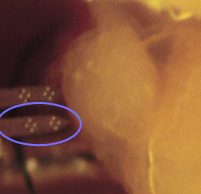
\includegraphics[width=0.25\textwidth]{shank.jpg}
	\caption{Shank with 8 electrodes (channels).}
	\label{fig:shank}
	\vspace{-10pt}
\end{wrapfigure}
In this exercise we will take a small part of real dataset HC-3\footnote{https://crcns.org/data-sets/hc/hc-3/about-hc-3}. The rat is running in a simple maze in which different visual markers are set up. The spiking activity of 311 neurons is recorded while rat is running in there. Among other things the $(x, y)$ position of the rat is recorded. In this exercise we will attempt to estimate position of the rat from the neuron activity data.

The original dataset is quite massive, so we will use only the data from one shank (see Figure \ref{fig:shank}) and this data will be pre-processed by the authors of the dataset. In \texttt{data} folder you can find two files: \texttt{ec012ec.187.fet.1} and \texttt{ec012ec.187.whl}. The first file is a matrix with 29 features and 89148 instances. After the feature extraction authors ended up with 29 features:
\begin{enumerate}[leftmargin=2cm]
\itemsep 0em
	\item [\texttt{1-3}] Three principal components, obtained using Principle Component Analysis (PCA)\footnote{\url{http://en.wikipedia.org/wiki/Principal_component_analysis}} of the data obtained form the channel 1.
	\item [\texttt{4-24}] PCA on channels 2 to 8, three main components per each.
	\item [\texttt{25}] Peak-to-trough on the channel of largest amplitude.
	\item [\texttt{26}] Peak-to-baseline on the channel of largest amplitude.
	\item [\texttt{27}] Trough-to-baseline on the channel of largest amplitude.
	\item [\texttt{28}] Spike duration.
	\item [\texttt{29}] Time moment. You will have to study \url{https://crcns.org/files/data/hc2/crcns-hc2-data-description.pdf} to find out what the sampling rate is.
\end{enumerate}
\ \\
The second file \texttt{ec012ec.187.whl} contains locations of two LEDs\footnote{\url{http://en.wikipedia.org/wiki/Light-emitting_diode}} placed on the mouse. The file \texttt{data/ec013.939.mpg.tar.gz} has an example of the video from which the location were extracted (this is not the same trial we work with in the exercise, so the trails do not match). There are 4 columns in this file
\begin{enumerate}
\itemsep 0em
	\item $X$ coordinate of the first LED.	
	\item $Y$ coordinate of the first LED.
	\item $X$ coordinate of the second LED.
	\item $Y$ coordinate of the second LED.
\end{enumerate}
We will use only the first LED.

Our goal is to to predict position of the rat only by looking by the features extracted from the neuronal activity. More details on how exactly we are going to do that are in the \texttt{codebase4.m} file. The result I got you can see on Figure \ref{fig:mousetrail}

\begin{figure}[H]
   \centering
   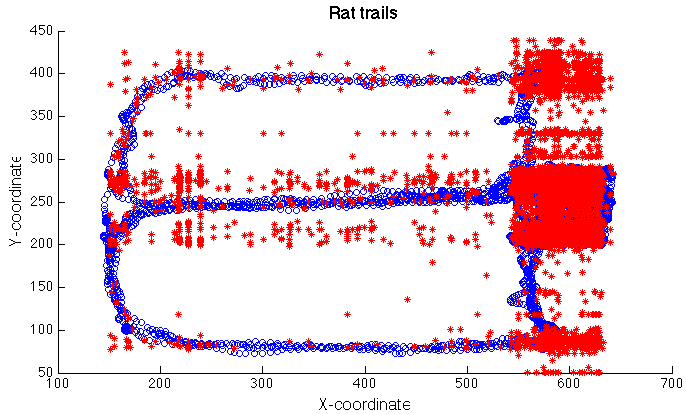
\includegraphics[width=1\textwidth]{trails.png} 
   \caption{Blue circles indicate true positions of the rat, red crosses -- predicted positions.}
   \label{fig:mousetrail}
\end{figure}
\ \\
In your report describe the logic behind the operations you are performing, results, plots and interpretations.
\end{exercise}

Previous exercises from this and previous sessions might have left you with a feeling that it is quite easy to achieve a result in neuroscience: you just think a little bit about the representation of your data, then use bunch of tools and the result is in your hands. The next exercise will give you the real feeling and give an opportunity to tackle with a problem.

%
% fMRI
%
\begin{exercise}{3}{PCA on fMRI data}{1+1*}
The most spatially precise non-invasive way of measuring brain activity is the Functional Magnetic Resonance Imaging (fMRI)\footnote{\url{http://en.wikipedia.org/wiki/Functional_magnetic_resonance_imaging}}. Things like reconstruction a video stream form the visual cortex has been attempted and successed\footnote{See for youself: \url{http://www.youtube.com/watch?v=nsjDnYxJ0bo}}.

\begin{wrapfigure}{r}{0.3\textwidth}
	\centering
	\vspace{-12pt}
	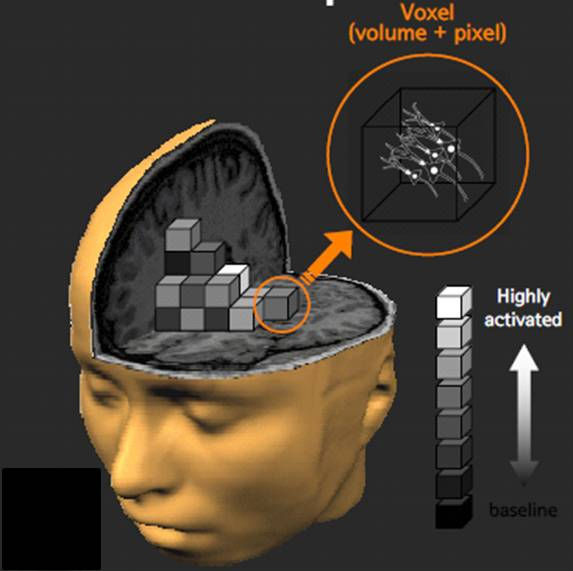
\includegraphics[width=0.3\textwidth]{voxel.jpg}
	\caption{Voxel.}
	\label{fig:voxel}
	\vspace{-10pt}
\end{wrapfigure}
The fMRI data is rather massive: at each moment of time (which is 1-2 seconds) the machine records the activity of $\approx$100,000 voxels (see Figure \ref{fig:voxel}). As you can imagine it is quite a challenge from computational point of view to analyze this kind of data.

In this exercise we will use the dataset\footnote{\url{https://crcns.org/data-sets/vc/vim-1/about-vim-1}}, where the region of the visual cortex ($\approx$25,000 voxels) was recorded while the test subject was looking at different images (see Figure \ref{fig:examplepic} for an example). The dataset consists of 1750 training instances and 120 test (validation) instances. We will be working with pre-processed data, which, nevertheless, has the size of 700\texttt{MB} (the orignial data is about 10\texttt{GB}).

In this exercise we apply PCA on this data to reduce it. The funny thing is, that you actually can throw more than half of it away without loosing any information at all. 

The codebase in the file \texttt{codebase4.m} will get you started. Go through the code and understand the logic of what is happening. Describe this logic in your report. Finish the code and run it, add pictures, plots and results what you get to the report.

\begin{figure}[H]
   \centering
   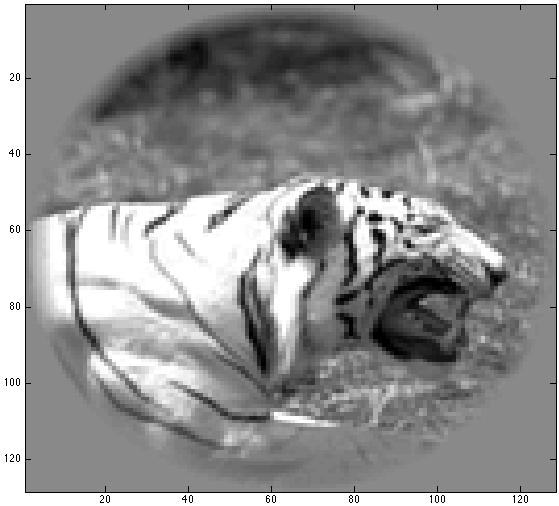
\includegraphics[width=0.4\textwidth]{examplepic.png} 
   \caption{An example of a stimulus.}
   \label{fig:examplepic}
\end{figure}

This is enough to get 1 point for this exercise. But since you are fascinated by the potential possibility of extracting visual information from the human brain you might want to continue and try to create an actual model, which will try to reconstruct images form the brain data. For that you will need to:
\begin{itemize}
\itemsep 0em
	\item Perform the PCA on images.
	\item Perform the PCA on features.
	\item Tranform test data into PC space using coefficients you obtained from PCA.
	\item Create a classifier.
	\item Evaluate the results.
\end{itemize}
I must warn you, that 
\begin{enumerate}
\itemsep 0em
	\item On average laptop building such a model with naive approach might take one day or so (10 hours on my laptop with 500 features and full images).
	\item If your reconstruction will show sky in light colors and land in dark color and everything else is not recognizable, this is already pretty good.
\end{enumerate}
Sufficient effort will be awarded with 1 bonus point.\\
\ \\
If you use Octave then you will need to install \texttt{statistics}\footnote{\url{http://octave.sourceforge.net/statistics/index.html}} package to run some functions we use. To do that open your Octave environment and type
\begin{verbatim}
> pkg install -forge io
> pkg install -forge statistics
\end{verbatim}

\end{exercise}


\begin{exercise}{4*}{Extract orientation}{1}
As you remember in the previous practice session we tried to identify orientation of the bar by looking at the neuronal activity of the rat. The dataset we used is \url{http://crcns.org/files/data/lgn-1/crcns_lgn-1_data_description.pdf}.

Your task is to take the data from the previous session and attempt to once more implement the whole pipeline of applying machine learning to the data:
\begin{enumerate}
\itemsep 0em
	\item Take the data and look at it. Read the description, study the values, etc. until you understand it.
	\item Take features are average spiking rates of neurons, so
	\item one instance will consist of 72 numbers. Spiking rate of each of the neurons during one trial. The minimal number of trial per neuron is 5, so you will have 5 trials per each stimulus.
	\item You will have 12 classes (12 orientations).
	\item Split dataset into training and test sets.
	\item Create a model using training set.
	\item Evaluate it's performance on the test set.
	\item Try to change something to increase the performance.
	\item Report what you did, what you got and interpret the results.
\end{enumerate}
\end{exercise}


\begin{exercise}{5}{Performance measures}{0.5}
Read about \emph{precision} and \emph{recall} (\url{http://en.wikipedia.org/wiki/Precision_and_recall}). Talk about true/false positives/negatives and how to compute precision and recall. Explain what is the intuition behind these concepts. Come up with an example where simple accuracy does not give reasonable evaluation of the model. Find any other performance measure, explain it and demonstrate how it is better on the same example where accuracy fails.
\end{exercise}
\ \\
\ \\
\ \\
\ \\
\ \\
Please submit a \texttt{pdf} report with answers to the questions and comments about your solutions. Also submit a code for the programming exercise(s). Pack those into \texttt{zip} archive and upload to the course web page.

\end{document}










